\begin{exercise}
      {ID-1eb9222643a140ed496faf37c4085ffc3b7839a8}
      {Benachbarte Kreise}
  \ifproblem\problem\par
    \begin{enumerate}[a)]
      \item \raisebox{-3.25\baselineskip}{%
            \begin{minipage}{0.25\linewidth}
              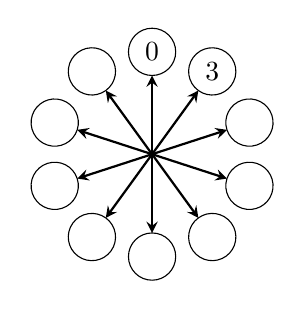
\begin{tikzpicture}
                \draw[line width=0.8pt, <->, >=stealth] (0, 1) -- (0, -1);
                \draw (0,  1.3) circle[radius=3mm] node{0};
                \draw (0, -1.3) circle[radius=3mm];
                \begin{scope}[rotate=36]
                  \draw[line width=0.8pt, <->, >=stealth] (0, 1) -- (0, -1);
                  \draw (0,  1.3) circle[radius=3mm];
                  \draw (0, -1.3) circle[radius=3mm];
                \end{scope}
                \begin{scope}[rotate=72]
                  \draw[line width=0.8pt, <->, >=stealth] (0, 1) -- (0, -1);
                  \draw (0,  1.3) circle[radius=3mm];
                  \draw (0, -1.3) circle[radius=3mm];
                \end{scope}
                \begin{scope}[rotate=108]
                  \draw[line width=0.8pt, <->, >=stealth] (0, 1) -- (0, -1);
                  \draw (0,  1.3) circle[radius=3mm];
                  \draw (0, -1.3) circle[radius=3mm];
                \end{scope}
                \begin{scope}[rotate=144]
                  \draw[line width=0.8pt, <->, >=stealth] (0, 1) -- (0, -1);
                  \draw (0,  1.3) circle[radius=3mm];
                  \draw (0, -1.3) circle[radius=3mm] node{3};
                \end{scope}
              \end{tikzpicture}
            \end{minipage}}\hfill
            \begin{minipage}[t]{0.74\linewidth}
              Die Zahlen 0, 1, 2, 3, 4, 5, 6, 7, 8, 9 sollen so in die kleinen Kreise
              der Abbildung eingetragen werden, dass jedes Paar benachbarter Kreise
              dieselbe Summe wie das Paar an den beiden entgegengesetzten Pfeilspitzen
              ergibt.\medskip\par
              Jede der zehn Zahlen soll genau einmal vorkommen. Die Zahlen 0 und 3
              sollen wie angegeben eingetragen werden.\medskip\par
              Gib eine Eintragung an, die alle diese Forderungen erfüllt!
            \end{minipage}
      \item Für die Zahlen 10, 11, 12, 13, 14, 15, 16, 17, 18, 19 läßt sich
            eine entsprechende Aufgabe stellen. Wie kann man für sie auf einfache
            Weise eine Lösung aus der Lösung von a) gewinnen?
      \item Löse die entsprechende Aufgabe für die natürlichen Zahlen
            $n$, $n+1$, $n+2$, $n+3$, $n+4$, $n+5$, $n+6$, $n+7$, $n+8$ und $n+9$.
    \end{enumerate}
  \fi
  %\ifoutline\outline\par
  %\fi
  %\ifoutcome\outcome\par
  %\fi
\end{exercise}
